%%%%%%%%%%%%%%%%%%%%%%%%%%%%%%%%%%%%%%%%%
% Beamer Presentation
% LaTeX Template
% Version 1.0 (10/11/12)
%
% This template has been downloaded from:
% http://www.LaTeXTemplates.com
%
% License:
% CC BY-NC-SA 3.0 (http://creativecommons.org/licenses/by-nc-sa/3.0/)
%
%%%%%%%%%%%%%%%%%%%%%%%%%%%%%%%%%%%%%%%%%

%----------------------------------------------------------------------------------------
%	PACKAGES AND THEMES
%----------------------------------------------------------------------------------------

\documentclass{beamer}
\mode<presentation> {
\usetheme{Madrid}
}
\usepackage{url}
\usepackage{lmodern}
\usepackage{graphicx}
\usepackage{booktabs}

% for mathematics
\usepackage{amsmath}
\usepackage{amsthm}

%----------------------------------------------------------------------------------------
%	TITLE PAGE
%----------------------------------------------------------------------------------------

\title[Financial mathematics with Python]{UROPS Project Presentation 8} % The short title appears at the bottom of every slide, the full title is only on the title page

\author{Wang Zexin} % Your name
\institute[NUS]
{
Chapter 18 Portfolio Valuation\\
of Python for Finance\\[3mm]
\medskip
\textit{Quantitative Finance\\
National University of Singapore\\}
}
\date{\today}

\begin{document}
%----------------------------------------------------------------------------------------
%	TITLE PAGE
%----------------------------------------------------------------------------------------
\begin{frame}
\titlepage
\end{frame}

%----------------------------------------------------------------------------------------
%	TABLE OF CONTENTS
%----------------------------------------------------------------------------------------

%------------------------------------------------
\begin{frame}
\frametitle{Today's Agenda}
\tableofcontents
\end{frame}

%------------------------------------------------
\begin{frame}
\frametitle{Changes due to different Python version}
We are using Python 3.6 while the version in the book is Python 2.7\\
So here is a list of items to change\\[2mm]
\begin{itemize}
	\item print x now becomes print(x)
	\item dict.iteritems() now becomes dict.items()
	\item xrange now becomes range
	\item lambda (k, v) : (v, k) is no longer available
	\item instead we can only use: lambda x : (x[1], x[0])
	\item x / 2 is float division, while x // 2 is integer division
\end{itemize}
\end{frame}

%------------------------------------------------
\section{General Modularization}

%------------------------------------------------
\begin{frame}
\frametitle{General Modularization}
The almost complete modularization of the analytics library:\\
(Based on Monte Carlo simulation being the only numerical method)
\begin{itemize}
	\item Discounting - $constant\_short\_rate$
	\item Relevant data - $market\_environment$
	\item Simulation objects
	\begin{itemize}
		\item geometric\_brownian\_motion
		\item jump\_diffusion
		\item square\_root\_diffusion
	\end{itemize}
	\item Valuation objects
	\begin{itemize}
		\item valuation\_mcs\_european
		\item valuation\_mcs\_american
	\end{itemize}
	\item Nonredundancy
	\item Correlations
	\item Positions
\end{itemize}
\end{frame}

\section{Derivatives Positions}

\subsection{Initialization}

%------------------------------------------------
\begin{frame}
\frametitle{Initializiation}
The derivatives positions class will include these attributes:
\begin{itemize}
	\item Quantity
	\item Underlying
	\item Market Environment (A $mar\_env$ object)
	\item Otype (which valuation class to use)
	\item Payoff function (A string with the formula for payoff)
\end{itemize}
\end{frame}

%------------------------------------------------
\begin{frame}
\frametitle{Derivatives Position}
\begin{figure}[H]
	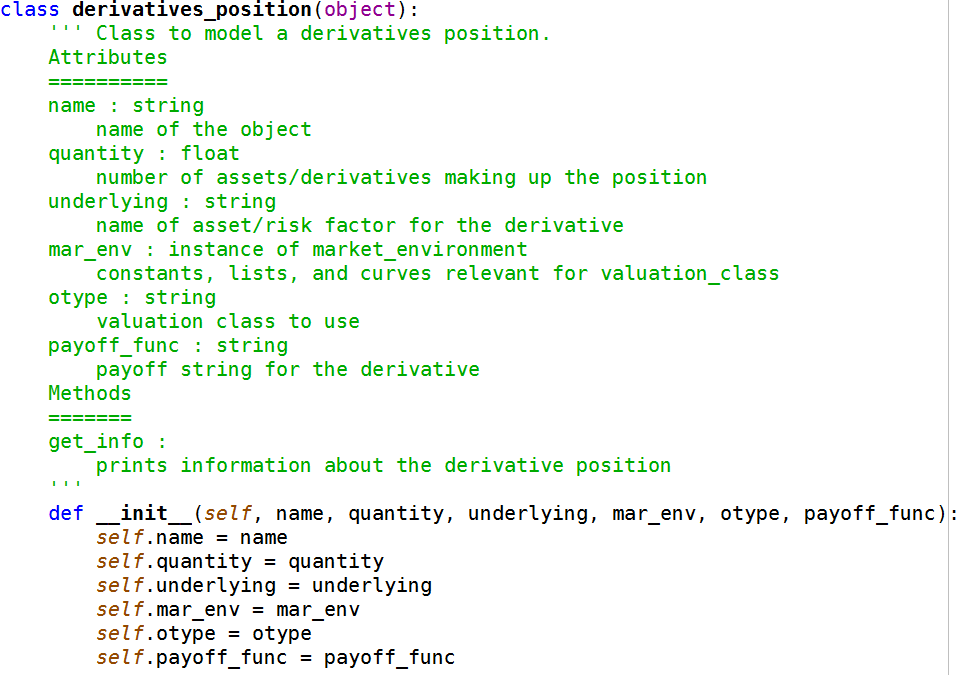
\includegraphics[scale=0.44]{derivatives_position_class.png}
\end{figure}
\end{frame}

\subsection{$get\_info$ method}
%------------------------------------------------
\begin{frame}
\frametitle{Derivatives Position}
This class also comes with a $get\_info$ method.\\
In which $payoff\_function$ is only a string for symbolic computations.
\begin{figure}[H]
	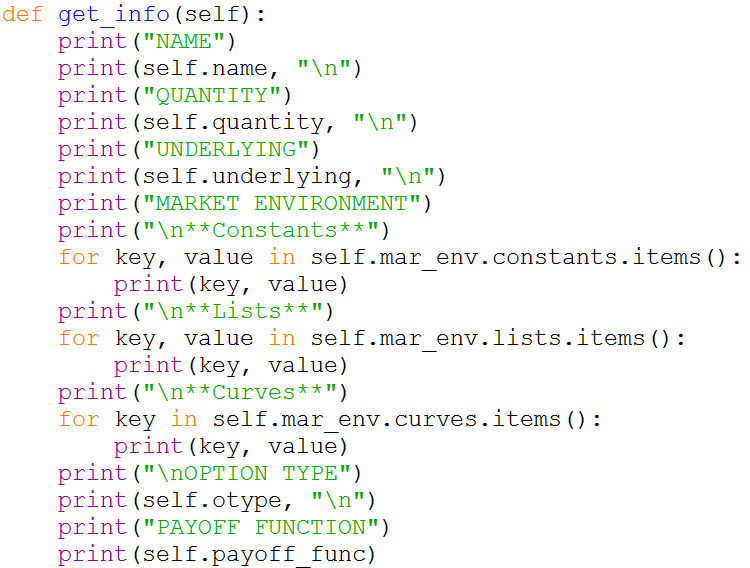
\includegraphics[scale=0.44]{derivatives_position_get_info.png}
\end{figure}
\end{frame}

\subsection{Use Case}
%------------------------------------------------
\begin{frame}
\frametitle{Derivatives Position - Use Case}
Here is a simple use case of the $derivatives\_position$ class.
\begin{figure}[H]
	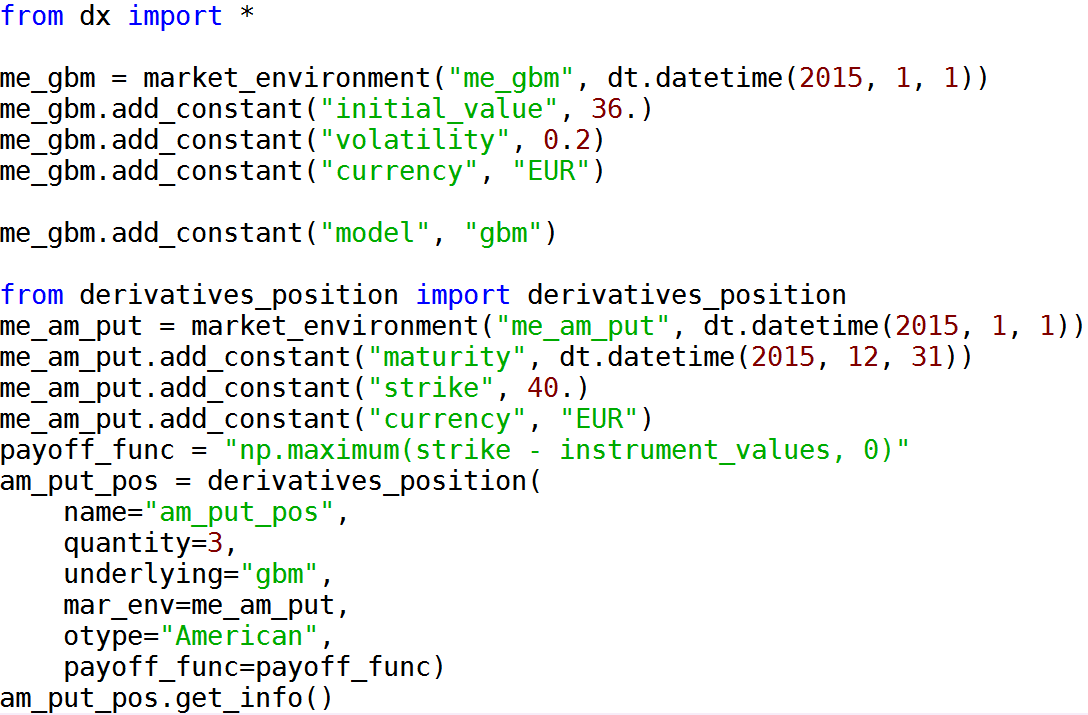
\includegraphics[scale=0.37]{derivatives_position_use_case.png}
\end{figure}
\end{frame}

\section{Derivatives Portfolio}
\subsection{Initialization}
%------------------------------------------------
\begin{frame}
\frametitle{Derivative Portfolio}
Initialization for the $derivatives\_portfolio$ class.
\begin{figure}
	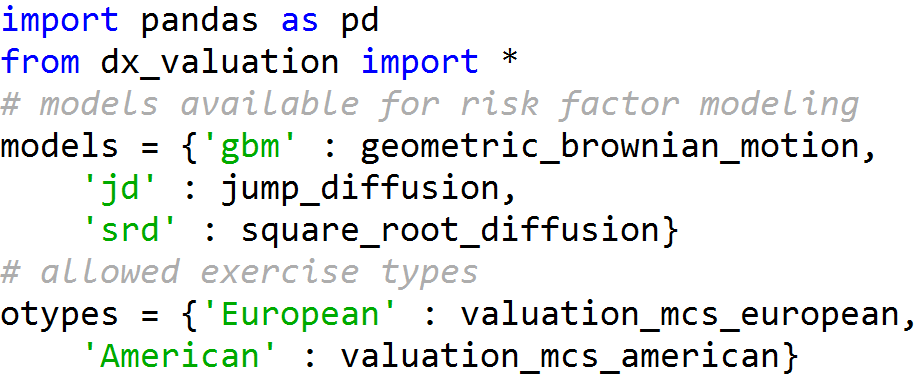
\includegraphics[scale=0.45]{derivatives_portfolio_init.png}
\end{figure}
\end{frame}

\subsection{Attributes}
%------------------------------------------------
\begin{frame}
\frametitle{Derivatives Portfolio}
The attributes of the $derivatives\_portfolio$ class are initialized as follows:
\begin{figure}[H]
	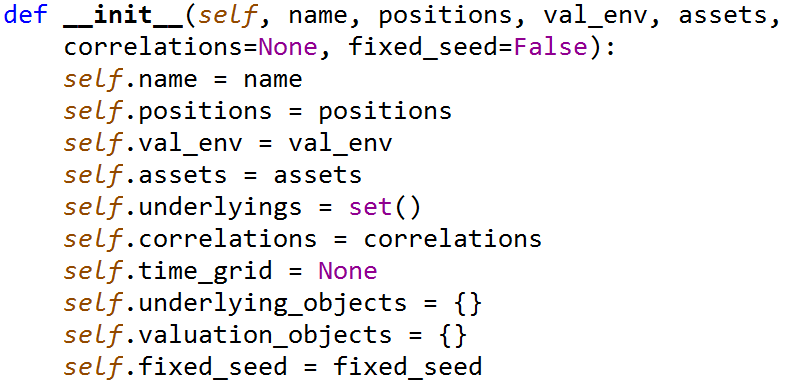
\includegraphics[scale=0.45]{derivatives_portfolio_attributes.png}
\end{figure}
\end{frame}

\subsection{Time Grid}
%------------------------------------------------
\begin{frame}
\frametitle{Derivatives Portfolio - Time Grid}
During initialization, the class would then go on to calculate the time grid.
\begin{figure}[H]
	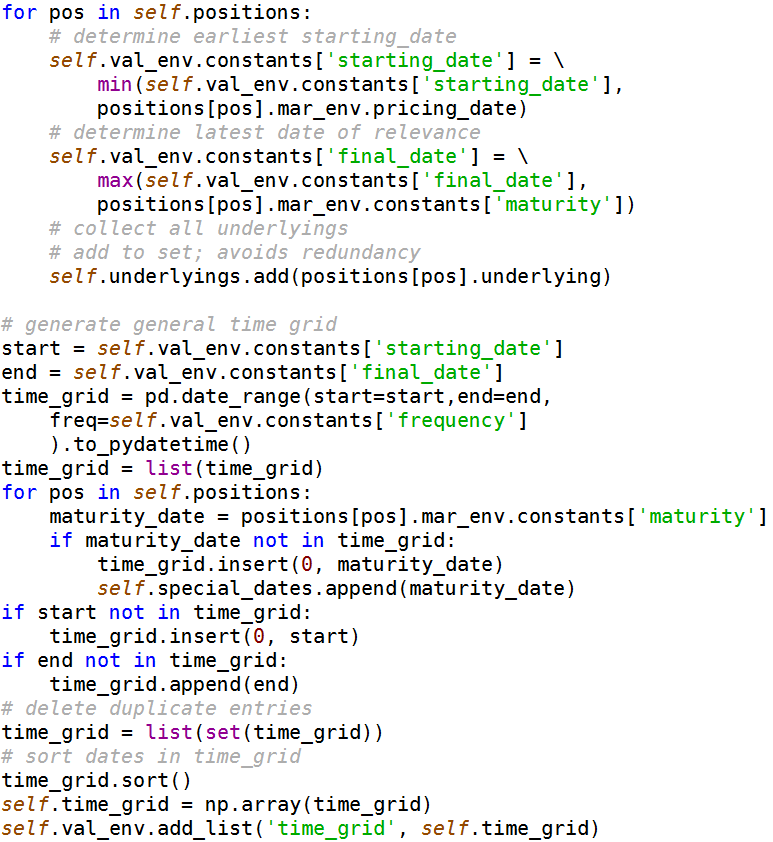
\includegraphics[scale=0.32]{derivatives_portfolio_time_grid.png}
\end{figure}
\end{frame}

\subsection{Cholesky Matrix}
%------------------------------------------------
\begin{frame}
\frametitle{Derivatives Portfolio - Cholesky Matrix}
If the correlation matrix is input in as a parameter, the class would calculate the Cholesky matrix during the initialization.
\begin{figure}[H]
	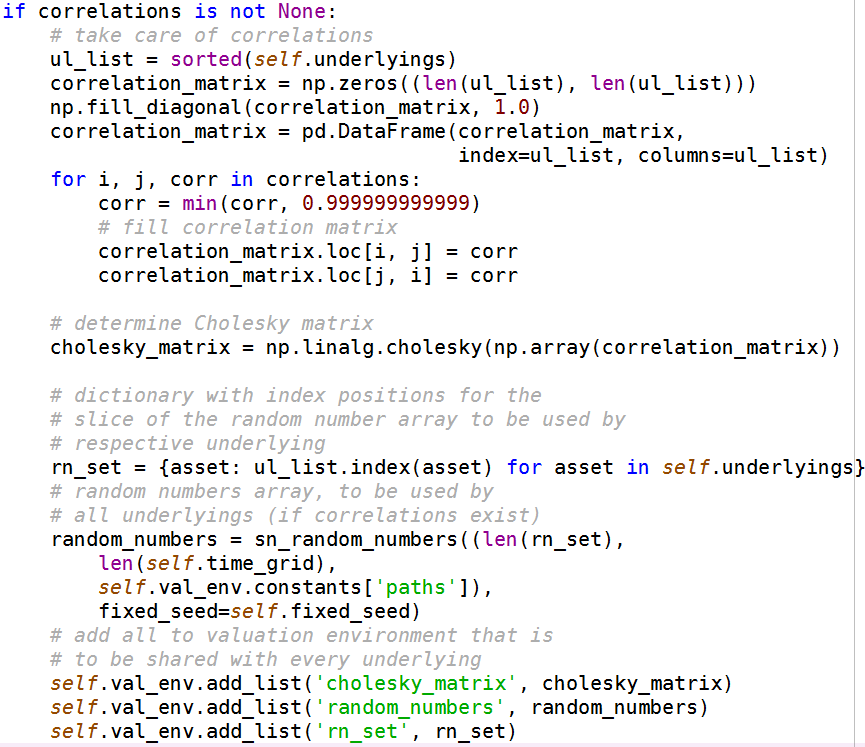
\includegraphics[scale=0.32]{derivatives_portfolio_cholesky_matrix.png}
\end{figure}
\end{frame}

\subsection{Positions}
%------------------------------------------------
\begin{frame}
\frametitle{Derivatives Portfolio - Positions}
The portfolio will contain the positions for derivatives as well.
\begin{figure}[H]
	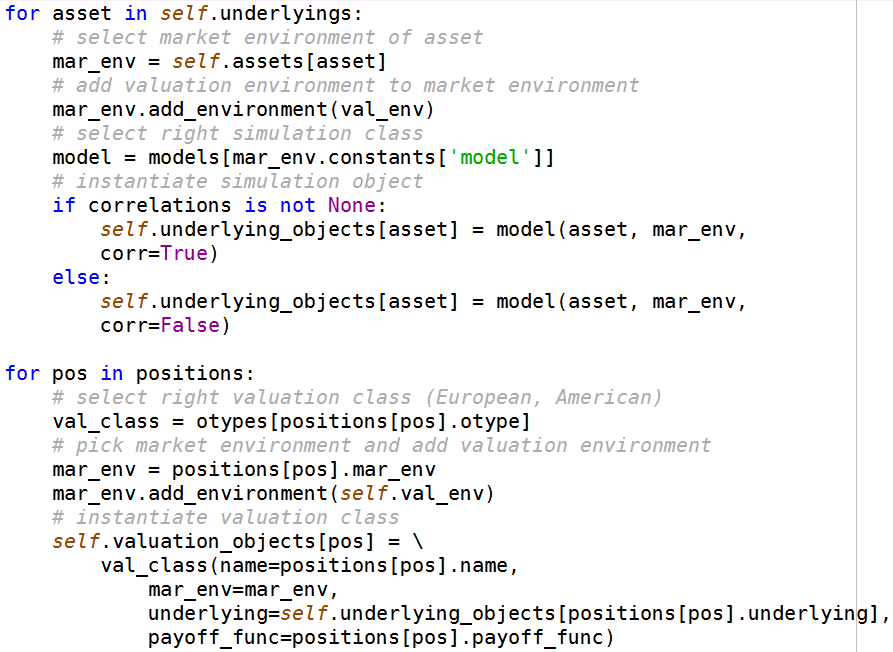
\includegraphics[scale=0.37]{derivatives_portfolio_underlying_positions.png}
\end{figure}
\end{frame}

\subsection{Getter methods}
%------------------------------------------------
\begin{frame}
\frametitle{Derivatives Portfolio - Getter methods}
The portfolio class comes with two convenient getters.
\begin{figure}[H]
	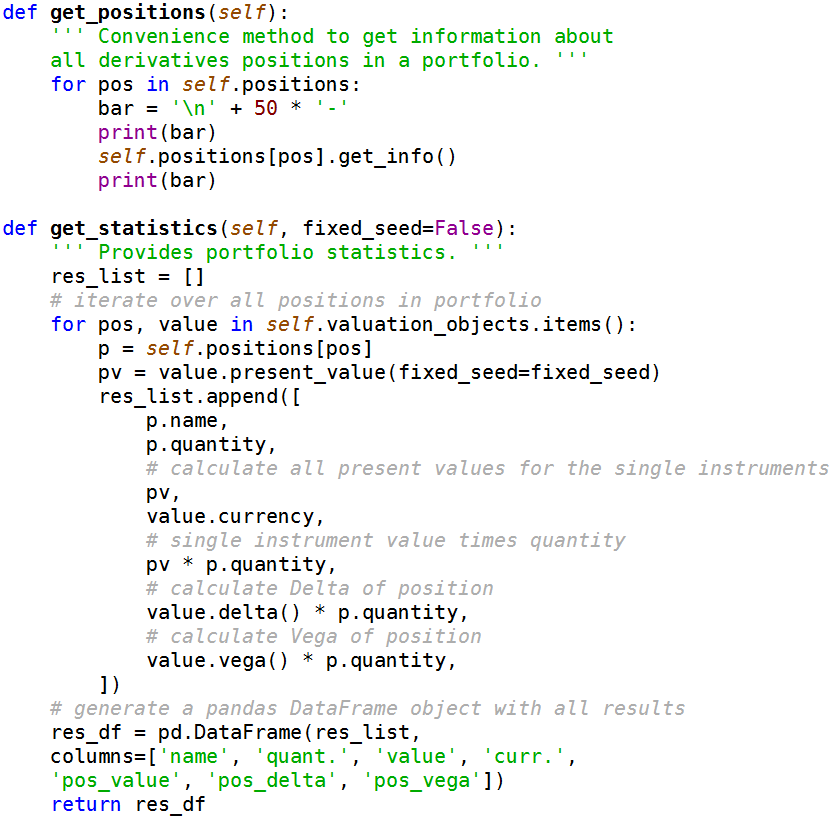
\includegraphics[scale=0.32]{derivatives_portfolio_getter_methods.png}
\end{figure}
\end{frame}

%------------------------------------------------
\begin{frame}
\frametitle{Derivatives Portfolio - Use Case}
A simple use case of the $derivatives\_portfolio$ class to build an object of the class first. Note that this use case comes directly after the use case of the previous $derivatives\_position$ class.
\begin{figure}[H]
	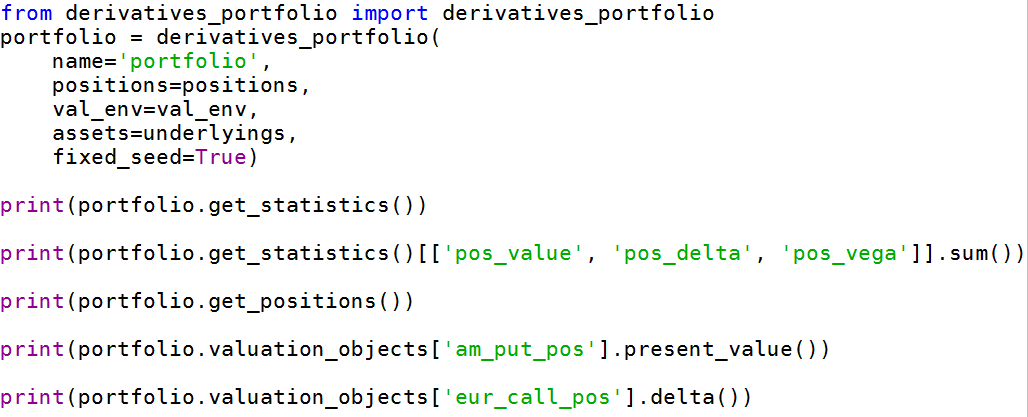
\includegraphics[scale=0.46]{derivatives_portfolio_use_case_1.png}
\end{figure}
\end{frame}

%------------------------------------------------
\begin{frame}
\frametitle{Derivatives Portfolio - Use Case}
This use case tests on whether the class can accept a correlation matrix correctly and build a cholesky matrix or not.
\begin{figure}[H]
	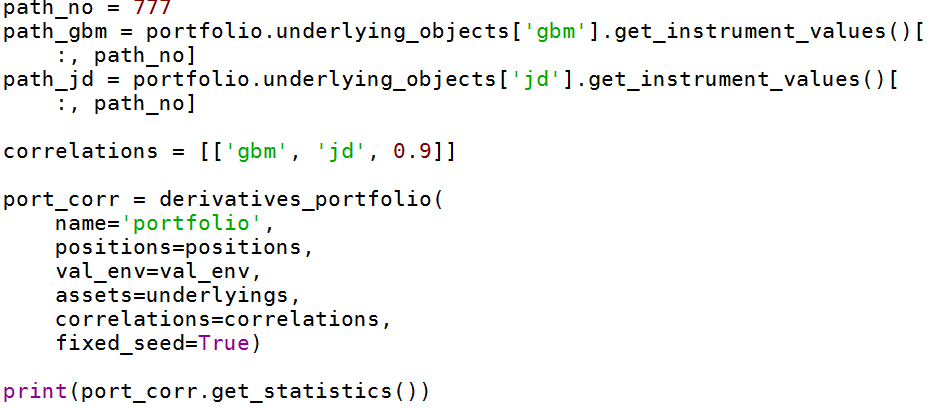
\includegraphics[scale=0.49]{derivatives_portfolio_use_case_2.png}
\end{figure}
\end{frame}

%------------------------------------------------
\begin{frame}
\frametitle{Derivatives Portfolio - Use Case}
This use case tests on the interaction between the components of the $derivatives\_portfolio$ class.
\begin{figure}[H]
	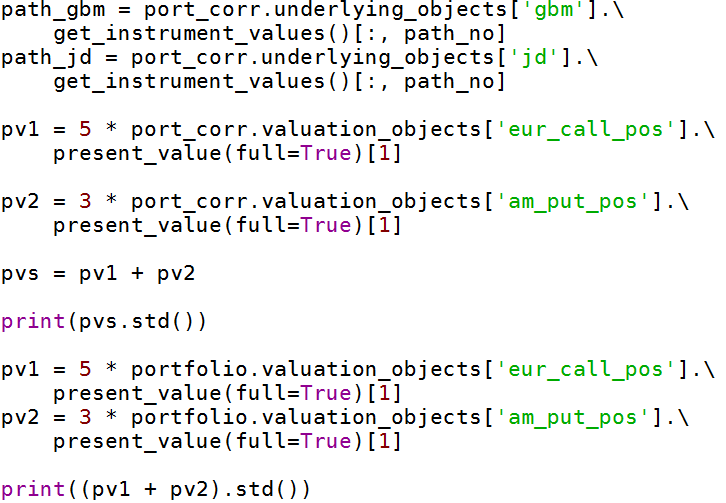
\includegraphics[scale=0.5]{derivatives_portfolio_use_case_3.png}
\end{figure}
\end{frame}

\section{Wrapper class}
%------------------------------------------------
\begin{frame}
\frametitle{Wrapper class - implementation}
\begin{figure}[H]
	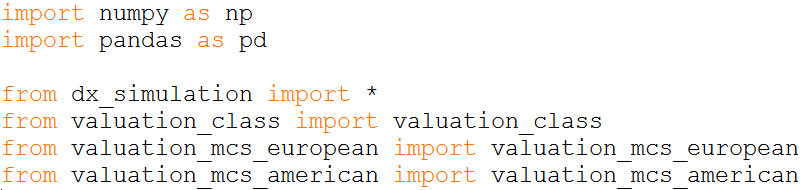
\includegraphics[scale=0.48]{wrapper_class.png}
\end{figure}
With this $dx\_library.py$, we are now able to import the valuation framework package for the derivatives portfolio as well the simulation classes in one line.
\end{frame}

%------------------------------------------------
\begin{frame}
\frametitle{Wrapper class - testing}
Now we need to enhance the $\_\_init\_\_.py$ which initially has the same content as $dx\_frame.py$,  $dx\_simulation.py$ and $dx\_valuation.py$ in the same directory to include importing the simulation classes.
\begin{figure}[H]
	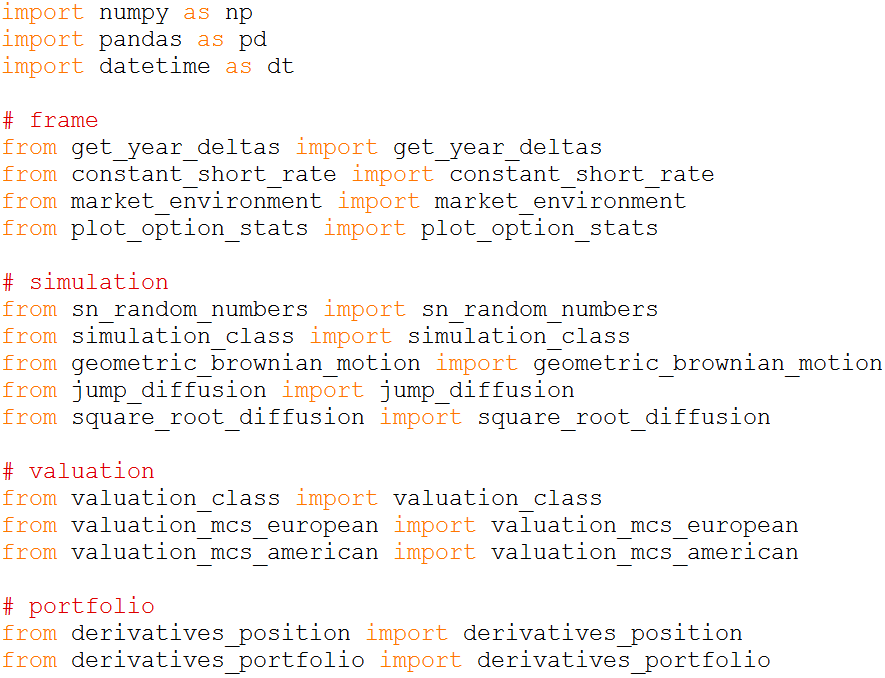
\includegraphics[scale=0.35]{overall_wrapper_class.png}
\end{figure}
\end{frame}

%-----------------------------------------------
\begin{frame}
\Huge{\centerline{Thank You}}
\begin{center}
\begin{normalsize}
\emph{E0007424@u.nus.edu}
\end{normalsize}
\end{center}
\end{frame}

%------------------------------------------------

\end{document} 